\chapter{Related Work}\label{chap:relatedwork}
%Give a brief overview of the work relevant for your thesis. 
\section{Self-supervised feature learning}
Self-supervised feature learning is a crucial process that identifies patterns within extensive unlabeled datasets without the need for human-annotated labels. Plenty of research has been done in this field in the recent years. Several methods have been proposed, each with unique mechanisms and varying levels of success.

\subsection{Contrastive learning}
Contrastive learning has gained significant attention for its effectiveness in self-supervised feature learning. One of the seminal works in this area is SimCLR~\cite{chen2020simple}, It employs a simple yet robust framework that leverages data augmentations to create positive pairs from the same image and negative pairs from different images. The model uses a contrastive loss to distinguish between these pairs, learning robust representations in the process. On the other hand, MoCo (Momentum Contrast)~\cite{he2020momentum} introduces a dynamic dictionary with a momentum encoder. This approach allows the model to maintain a queue of negative samples, effectively reducing memory requirements and improving scalability. Nevertheless, it still requires a substantial number of negative samples to function optimally and necessitates careful tuning of the momentum parameter to balance stability and learning efficiency.

\subsection{Clustering-based feature learning}
Clustering-based feature learning approaches automatically uncover the natural groupings of data within the latent representation space. This clustering process helps in understanding the inherent structure of the data by grouping similar data points together based on learned features. Agglomerative Clustering with Self-supervision~\cite{asano2020selflabelling} can capture multi-scale structures and found to be effective for diverse datasets. But found to be computationally expensive and needs careful tuning of the self-supervised task. SwAV~\cite{caron2021unsupervised} combines clustering with contrastive learning by swapping assignments between different augmented views of the image. This method is efficient in terms of computational resources and achieves state-of-the-art performance on several benchmarks. But it is sensitive to the choice of hyperparameters.

\subsection{Distillation-based methods}
Distillation-based methods have also shown considerable promise in self-supervised learning. BYOL (Bootstrap Your Own Latent)~\cite{grill2020bootstrap} introduces a teacher-student network where the student learns to predict the teacher's representations. Remarkably, BYOL achieves this without using negative samples, simplifying the training process and reducing computational demands. However, it is sensitive to the choice of data augmentations and network architecture, and there is a potential risk of model collapse if not properly tuned. DINO~\cite{caron2021emerging}, extends the self-distillation approach to Vision Transformers~\cite{dosovitskiy2020image}. DINO captures global image representations effectively without relying on negative samples. It shows strong performance on object detection and segmentation tasks, showcasing the potential of transformers in self-supervised learning.

Unlike these unsupervised representation learning efforts, our research revolves around CutLER~\cite{wang2023cut}, which focuses on automatically identifying natural pixel groupings and detecting instances within each image.

\section{Unsupervised object detection and instance segmentation}
If we consider the recent methods for unsupervised object detection semantic segmentation, most of them leverage on self-supervised Vision Transformer(ViT)~\cite{dosovitskiy2020image} features. In DINO~\cite{caron2021emerging} it is observed that the underlying semantic segmentation of images can be extracted using the saliency maps from the ViT. 

The quality of this segmentation is superior to the existing methods if the image contains only is one instance. The superiority of DINO features to separate foreground and background has been affirmed by later works~\cite{engstler2023understanding}. Building on this observation, both LOST ~\cite{simeoni2021localizing} and TokenCut~\cite{wang2022tokencut} utilize DINO features to segment a single salient object from each image. These methods capitalize on the strength of DINO to construct a graph from the features of image patches. Unlike TokenCut and DINO, which can only detect one instance, LOST is capable of finding multiple instances within an image. But it can't be used as a pre-trained model for down stream tasks. But CutLER~\cite{wang2023cut} not only can detect multiple instances, the model can be further used as a pretrained model for label-efficient and fully-supervised learning.

FreeSOLO~\cite{wang2022freesolo} and the follow up work Exemplar-FreeSOLO~\cite{Ishtiak_2023_CVPR} (with its addition of a randomly drawn pool of exemplars used in a contrastive learning loss) generates coarse segmentation masks with low guality and refines it further through self training similar to CutLER. But the poor quality of the coarse maps is a major draw back of this method, where as CutLER masks made by the MaskCut~\cite{wang2023cut, wang2022tokencut} algorithm are usually better in quality and quantity than the initial masks used by MaskDistill~\cite{vangansbeke2022discovering} and \cite{wang2022freesolo}. Even though Maskdistill produces similar quality masks compared to MaskCut, as it only produces one class agnostic mask per image and MaskCut produces N fixed number of masks per image to use as pseudo labels, MaskCut weighs over Maskdistill in quantity.

As CutLER dominates in most cases, including producing better pseudo ground truth masks, ability to detect multiple instances, compatibility with various detection architectures, usable as pretrained model for supervised detection, our work would mostly focus on studying and improving the performance of CutLER.

\section{Semi-supervised object detection and instance segmentation}
Semi-supervised learning leverages both unlabeled data and a fraction of labeled data to improve the performance of models. In the context of object detection and semantic segmentation, several recent works have explored various techniques to enhance these tasks.

Most of the recent works in this domain includes a student-teacher model as in  Adaptive Teacher~\cite{Li_2022_CVPR}, Unbiased Teacher~\cite{liu2021unbiasedteachersemisupervisedobject} and Soft Teacher~\cite{xu2021endtoendsemisupervisedobjectdetection}. These methods slightly differ in the type of augmentations(strong, weak and hybrid augmentation) used and the method of action on the pseudo labels. For instance, Unbiased teacher addresses bias in pseudo-labeling by using a teacher-student model. The teacher generates pseudo-labels which are then used to train the student. The process iterates with the student eventually replacing the teacher. Where as the Soft teacher leverages both hard and soft pseudo-labels. The method uses a teacher model to generate soft labels (probabilistic outputs) for unlabeled data, which are used to train a student model.

%\input{Images/main/correspondences}
\begin{figure*}
	\centering
	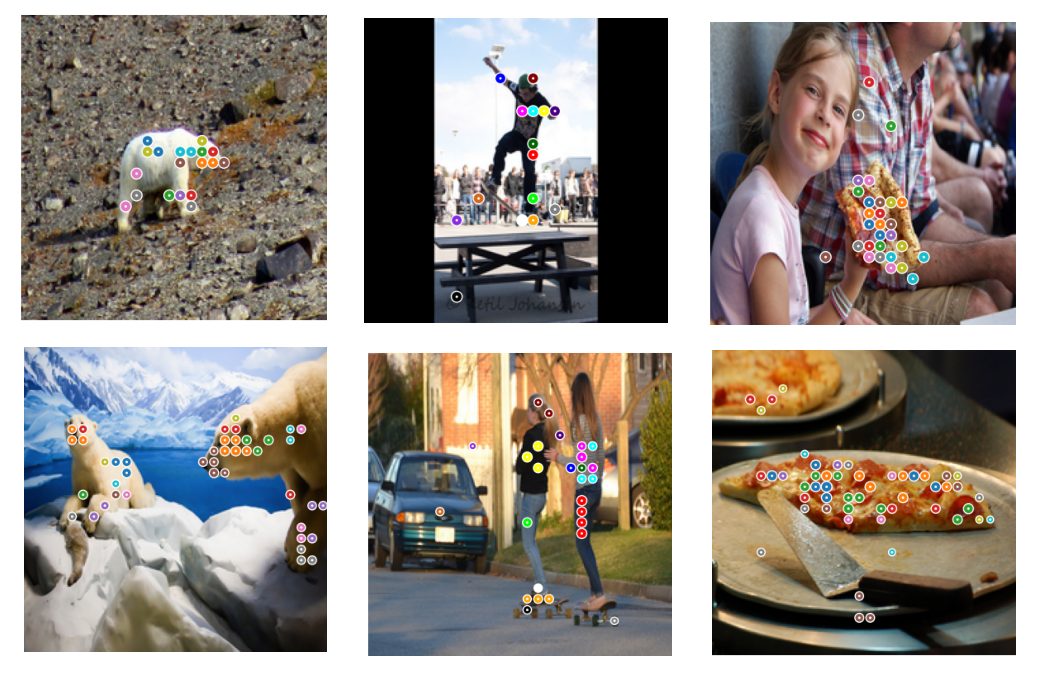
\includegraphics[width=0.95\textwidth]{Images/main/correspondences.png}
	\caption[\textbf{Keypoint correspondecences using relaxed best buddies}]{\textbf{Keypoint correspondecences using relaxed best buddies}. Prototype images at the top and query images at the bottom. Same colored points represent similar features }
	\label{fig:correspondecences}
\end{figure*}

Unlike relying on augmentations like most recent semi-supervised works, we tried to extract instances using keypoint correspondences taking inspiration from the Superglue~\cite{sarlin2020supergluelearningfeaturematching} paper. But the main challenge was instead of working with images taken two different perspectives, we are dealing with entirely different pair of images with similar instances.

Figure~\ref{fig:correspondecences} shows the keypoint correspondences between the prototype and query images. The correspondence is calculated by applying the relaxed best buddy algorithm on the descriptors corresponding to the foreground part of the prototype and query images, which is selected by applying a threshold on the saliency map. We relaxed the original best buddy algorithm~\cite{Aberman_2018} to extract more correspondence points enough to form a graph to perform graph-cut similar to~\cite{wang2022tokencut, sarlin2020supergluelearningfeaturematching}. We explored our options to geometrically separate the instances using the semantic information in the correspondences. But as we were unable to find a promising approach or inspiration from our research. For instance, Integer programming for multidimensional assignment problem~\cite{WALTEROS2014553} has a strict initial graph specification which restrict us to adapt it to our problem.

By considering the limitations of implementing a semi-supervised method using keypoint correspondences, we focus mostly on improving the unsupervised instance detection and segmentation by diving into the current state-of-the-art method CutLER~\cite{wang2023cut}; exploring it's limitations and ways to improve them.
 
% \todo{see if you included all literature work for Vision Transformer for Semantic Segmentation}
% \todo{ add little bit about Hierarchical Vision Transformer for say swin, satrt with where all hierarchy in transformer have been explored and in semnatic segmentation where all it fanne dout well}
% \todo{Then in the the section say a very little about groupVit and that you would be moving on to that and our ork builds on that }

% \section{Visual Grouping}

% \section{Visual Language Pretraining}
% Vision-language pretraining has emerged as a powerful paradigm, driving advancements in the intersection of vision and language understanding. By jointly modeling visual and textual modalities, these pretrained models have revolutionized a range of vision-language tasks. Vision-language pretraining involves training a joint model on a vast corpus of image and text data. By learning from the paired visual and textual information, the model gains a comprehensive understanding of the cross-modal relationships between images and their associated captions or descriptions. 

% Explain the math and notation.